\documentclass[pdftex,12pt, oneside]{article}

%\usepackage[paperwidth=8.5in, paperheight=13in]{geometry} % Folio
\usepackage[paperwidth=8.27in, paperheight=11.69in]{geometry} % A4

\usepackage{makeidx}         % allows index generation
\usepackage{graphicx}        % standard LaTeX graphics tool
                             % when including figure files
\usepackage[bottom]{footmisc}% places footnotes at page bottom
\usepackage[english]{babel}
\usepackage{enumerate}
\usepackage{paralist}
\usepackage{float}
\usepackage{gensymb}  
\usepackage{listings}
\usepackage{color}
\usepackage{mathtools} % atau \usepackage{amsmath}
\renewcommand{\baselinestretch}{1.5}

\newcommand{\HRule}{\rule{\linewidth}{0.5mm}}

\definecolor{codegreen}{rgb}{0,0.6,0}
\definecolor{codegray}{rgb}{0.5,0.5,0.5}
\definecolor{codepurple}{rgb}{0.58,0,0.82}
\definecolor{backcolor}{rgb}{0.95,0.95,0.92}

\lstdefinestyle{mystyle}{
  backgroundcolor=\color{backcolor},
  commentstyle=\color{codegreen},
  keywordstyle=\color{magenta},
  stringstyle=\color{codepurple},
  basicstyle=\footnotesize,
  breakatwhitespace=false,
  breaklines=true,
  captionpos=b,
  keepspaces=true,
  numbers=left,
  numbersep=5pt,
  showspaces=false,
  showstringspaces=false,
  showtabs=false,
  tabsize=2
}

\lstset{style=mystyle}


\begin{document}
\sloppy % biar section ga melebar melewati kertas

\begin{center}
{\large RANCANGAN SISTEM \textit{WEB SERVICES} SEBAGAI CARA KOMUNIKASI DENGAN TEMPAT PEMBAYARAN DALAM PENCATATAN PEMBAYARAN PAJAK BUMI DAN BANGUNAN PERDESAAN DAN PERKOTAAN DI KABUPATEN BREBES.}
\\[1cm]
DD MMM 2016\\
Priyanto Tamami, S.Kom.
\end{center}

%\frontmatter%%%%%%%%%%%%%%%%%%%%%%%%%%%%%%%%%%%%%%%%%%%%%%%%%%%%%%


%%%%%%%%%%%%%%%%%%%%%%%%%%%%%%%%%%%%%%%%%%%%%%%%%%%%%%%%%%%%%%%%%%%%%%

\section{TUJUAN SISTEM}

Tujuan dari dibangunnya sistem \textit{web services} ini adalah mempermudah pencatatan transaksi pembayaran yang terjadi melalui Bank agar tersimpan pada basis data Sistem Manajemen Informasi Objek Pajak PBB-P2.


\section{PEMODELAN SISTEM}

Sistem akan dimodelkan sebagai bentuk \textit{web services} yang menerima 3 (tiga) bentuk masukan, yaitu untuk melakukan \textit{inquiry}, pencatatan pembayaran, dan \textit{reversal}.

Karena perangkat pemrograman yang digunakan nantinya mendukung pemrograman berorientasi objek, maka akan lebih mudah apabila pendekatan pemodelan menggunakan \textit{Unified Modeling Language} (UML). Bentuk-bentuk diagram yang akan digunakan adalah sebagai berikut :

\begin{enumerate}
  \item Diagram \textit{Use-Case}
  
  Diagram ini akan mengilustrasikan gambaran utuh sebuah sistem yang berinteraksi dengan pengguna.
  
  \item Diagram \textit{Activity}
  
  Diagram ini akan mengilustrasikan aktifitas dari tiap objek yang saling berinteraksi membentuk sebuah sistem yang menerima masukkan, memprosesnya, dan kemudian menghasilkan sebuah keluaran yang dibutuhkan.
  
  \item Diagram \textit{Class}
  
  Diagram ini akan mengilustrasikan kelas-kelas pembentuk sistem berdasarkan objek-objek yang teridentifikasi sebelumnya.
  
  \item Diagram \textit{Sequence}
  
  Diagram ini akan mengilustrasikan alur interaksi dari tiap kelas berdasarkan skenario tertentu.
  
\end{enumerate}

Lebih detail mengenai diagram-diagram tersebut akan dijelaskan sebagai berikut.


\subsection{Diagram \textit{Use-Case}}

Diagram \textit{Use-Case} ini akan menjelaskan gambaran menyeluruh atau gambaran besar aktifitas antara pengguna dengan sistem yang dibangun. Diagram \textit{Use-Case} pada sistem ini seperti terlihat pada gambar \ref{fig:uml-use-case} :

\begin{figure}[H]
  \centering
  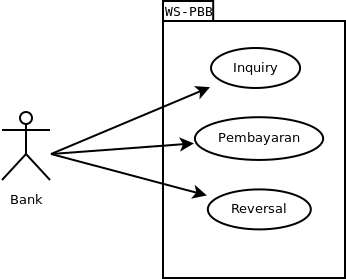
\includegraphics[width=0.5\textwidth]{./resources/uml/uml-use-case}
  \caption{Diagram \textit{Use-Case} Sistem \textit{Web Services} Pencatatan Pembayaran PBB-P2}
  \label{fig:uml-use-case}
\end{figure}

Yang menjadi aktor disini adalah Bank dalam artian \textit{client} yang akan melakukan akses ke sistem \textit{web services} pencatatan pembayaran Pajak Bumi dan Bangunan Perdesaan dan Perkotaan (PBB-P2).

Akses yang dapat dilakukan oleh \textit{client} ada 3 (tiga) skenario, yaitu \textit{Inquiry}, Pembayaran, dan \textit{Reversal}

\textit{Inquiry} ini adalah permintaan informasi PBB-P2 Terhutang oleh \textit{client} ke \textit{server web services}. Skenario Pembayaran adalah permintaan dari \textit{client} ke \textit{server web services} untuk melakukan pencatatan pembayaran PBB-P2 berdasarkan Nomor Objek Pajak (NOP) dan Tahun Pajak yang akan dicatatkan pembayarannya. Sedangkan skenario \textit{reversal} adalah permintaan oleh \textit{client} ke \textit{server web services} untuk melakukan pembatalan pencatatan pembayaran yang telah dilakukan.

\subsection{Diagram \textit{Activity}}

Diagram \textit{Activity} ini 

\subsubsection{Diagram \textit{Activity} Untuk Skenario \textit{Inquiry}}
\subsubsection{Diagram \textit{Activity} Untuk Skenario Pencatatan Pembayaran}
\subsubsection{Diagram \textit{Activity} Untuk Skenario \textit{Reversal}}
\subsection{Diagram \textit{Class}}
\subsection{Diagram \textit{Sequence}}
\subsubsection{Diagram \textit{Sequence} Untuk Skenario Konfigurasi \textit{Spring Framework}}
\subsubsection{Diagram \textit{Sequence} Untuk Skenario \textit{Inquiry} Gagal Karena Tahun Pajak Bukan Angka}
\subsubsection{Diagram \textit{Sequence} Untuk Skenario \textit{Inquiry} Gagal Karena Data Tidak Ditemukan}
\subsubsection{Diagram \textit{Sequence} Untuk Skenario \textit{Inquiry} Gagal Karena Kesalahan Server}
\subsubsection{Diagram \textit{Sequence} Untuk Skenario \textit{Inquiry} Yang Sukses}
\subsubsection{Diagram \textit{Sequence} Untuk Skenario Transaksi Pembayaran Gagal Karena Jam Pembayaran Melebihi Jam Pencatatan}
\subsubsection{Diagram \textit{Sequence} Untuk Skenario Transaksi Pembayaran Gagal Karena Tagihan Telah Terbayar Atau Nihil}
\subsubsection{Diagram \textit{Sequence} Untuk Skenario Transaksi Pembayaran Gagal Karena Telah Dibatalkan}
\subsubsection{Diagram \textit{Sequence} Untuk Skenario Transaksi Pembayaran Gagal Karena Kesalahan Server}
\subsubsection{Diagram \textit{Sequence} Untuk Skenario Transaksi Pembayaran Yang Sukses}
\subsubsection{Diagram \textit{Sequence} Untuk Skenario \textit{Reversal} Gagal Karena Data Yang Diminta Tidak Ada}
\subsubsection{Diagram \textit{Sequence} Untuk Skenario \textit{Reversal} Gagal Karena Ada Data Pembayaran Yang Tercatat Ganda}
\subsubsection{Diagram \textit{Sequence} Untuk Skenario \textit{Reversal} Gagal Karena Kesalahan Server}
\subsubsection{Diagram \textit{Sequence} Untuk Skenario \textit{Reversal} Yang Sukses}


\section{AKTIVITAS PEMROSESAN DATA}

\begin{verbatim}
  Isinya :
    - output terpenting (goal)
    - identifikasi input 
    - alur pemrosesan data
  Arahnya ke unit testing
\end{verbatim}


\end{document}